\documentclass{article}

\usepackage{fancyhdr}
\usepackage{extramarks}
\usepackage{boondox-cal}
\usepackage{amsmath}
\usepackage{amsthm}
\usepackage{amsfonts}
\usepackage{tikz}
\usepackage[plain]{algorithm}
\usepackage{algpseudocode}

\usetikzlibrary{automata,positioning, arrows.meta}

%
% Basic Document Settings
%

\topmargin=-0.45in
\evensidemargin=0in
\oddsidemargin=0in
\textwidth=6.5in
\textheight=9.0in
\headsep=0.25in

\linespread{1.1}

\pagestyle{fancy}
\lhead{\hmwkAuthorName}
\chead{\hmwkClass\ (\hmwkClassInstructor): \hmwkTitle}
\rhead{\firstxmark}
\lfoot{\lastxmark}
\cfoot{\thepage}

\renewcommand\headrulewidth{0.4pt}
\renewcommand\footrulewidth{0.4pt}

\setlength\parindent{0pt}

%
% Create Problem Sections
%

\newcommand{\enterProblemHeader}[1]{
    \nobreak\extramarks{}{Problem \arabic{#1} continued on next page\ldots}\nobreak{}
    \nobreak\extramarks{Problem \arabic{#1} (continued)}{Problem \arabic{#1} continued on next page\ldots}\nobreak{}
}

\newcommand{\exitProblemHeader}[1]{
    \nobreak\extramarks{Problem \arabic{#1} (continued)}{Problem \arabic{#1} continued on next page\ldots}\nobreak{}
    \stepcounter{#1}
    \nobreak\extramarks{Problem \arabic{#1}}{}\nobreak{}
}

\setcounter{secnumdepth}{0}
\newcounter{partCounter}
\newcounter{homeworkProblemCounter}
\setcounter{homeworkProblemCounter}{1}
\nobreak\extramarks{Problem \arabic{homeworkProblemCounter}}{}\nobreak{}

%
% Homework Problem Environment
%
% This environment takes an optional argument. When given, it will adjust the
% problem counter. This is useful for when the problems given for your
% assignment aren't sequential. See the last 3 problems of this template for an
% example.
%
\newenvironment{homeworkProblem}[1][-1]{
    \ifnum#1>0
        \setcounter{homeworkProblemCounter}{#1}
    \fi
    \section{Problem \arabic{homeworkProblemCounter}}
    \setcounter{partCounter}{1}
    \enterProblemHeader{homeworkProblemCounter}
}{
    \exitProblemHeader{homeworkProblemCounter}
}

%
% Homework Details
%   - Title
%   - Due date
%   - Class
%   - Section/Time
%   - Instructor
%   - Author
%

\newcommand{\hmwkTitle}{Note\ \#1}
\newcommand{\hmwkDueDate}{February 28, 2024}
\newcommand{\hmwkClass}{Compiler}
\newcommand{\hmwkClassInstructor}{ant-hengxin}
\newcommand{\hmwkAuthorName}{\textbf{0130}}

%
% Title Page
%

\title{
    \vspace{2in}
    \textmd{\textbf{\hmwkClass:\ \hmwkTitle}}\\
    \vspace{0.1in}\large{\textit{\hmwkClassInstructor}}
    \vspace{3in}
}

\author{\hmwkAuthorName}
\date{}

\renewcommand{\part}[1]{\textbf{\large Part \Alph{partCounter}}\stepcounter{partCounter}\\}

%
% Various Helper Commands
%

% Useful for algorithms
\newcommand{\alg}[1]{\textsc{\bfseries \footnotesize #1}}

% For derivatives
\newcommand{\deriv}[1]{\frac{\mathrm{d}}{\mathrm{d}x} (#1)}

% For partial derivatives
\newcommand{\pderiv}[2]{\frac{\partial}{\partial #1} (#2)}

% Integral dx
\newcommand{\dx}{\mathrm{d}x}

% Alias for the Solution section header
\newcommand{\solution}{\textbf{\large Solution}}

% Probability commands: Expectation, Variance, Covariance, Bias
\newcommand{\E}{\mathrm{E}}
\newcommand{\Var}{\mathrm{Var}}
\newcommand{\Cov}{\mathrm{Cov}}
\newcommand{\Bias}{\mathrm{Bias}}

% empty underline
\newcommand{\emptyunderline}{\underline{\ \ \ \ \ \ }}

\begin{document}

\maketitle

\pagebreak

Big Picture:
\\

we are used to expressing lexical rules in regular expressions,
but we are writing the lexical analyzer through a \texttt{DFA}.\@ That means
that there exists some way to convert from regular expressions to \texttt{DFA}.\@
\[
    \texttt{re} \to \texttt{DFA}
\]

But this approach is overly complicated, and for simplicity's sake, let's do this thing in multiple steps:

%% TODO!

\[
  \texttt{re} \xrightarrow[\text{Construction}]{\text{Thompson}} \texttt{NFA} \xrightarrow[\text{Construction}]{\text{Subset}} \tikz[baseline=-0.5ex]{\node[inner sep=0] (DFA) {\texttt{DFA}}; \draw[-{Stealth[scale=0.8]}] (DFA) to[out=45,in=135,loop] (DFA);}
\]

And we also want to know how to convert a \texttt{DFA} to a \texttt{re}.
\\

Alphabet \( \Sigma \): A set of finite symbols.
\\

String \texttt{s} over alphabet \( \Sigma \): A sequence of symbols from \( \Sigma \). A special string \( \epsilon \) is the empty string with the property \( |\epsilon| = 0 \).
\\

\textbf{String operation}: concatenation: \texttt{x = dog, y = house} \( \Rightarrow \) \texttt{xy = doghouse}.
\\

Language \( L \) over alphabet \( \Sigma \): A countable set of strings over \( \Sigma \).
\\

\textbf{Language operation}:
\\

Suppose \texttt{L, M} are languages, we can use set operations to construct new languages:

\begin{enumerate}
    \item \texttt{L \( \cup \) M:= \{ s | s \( \in \) L or s \( \in \) M \} }
    \item \texttt{LM:= \{ s \( \in \) L and s \( \in \) M \}}
    \item \texttt{L\(^*\):= \( \bigcup_{i=0}^{\infty} \) L\(^i\) (Kleene closure) }
    \item \texttt{L\(^+\):= \( \bigcup_{i=1}^{\infty} \) L\(^i\) (Positive closure) }
\end{enumerate}

The following logic is, we firstly talk about the definition
of regular expression, then we talk about the definition of 
non-deterministic finite automaton (NFA), and we define what's the meaning
of a regular expression is equivalent to a NFA.\@
\\

\textbf{Regular expression}:
\\

A regular expression over alphabet \( \Sigma \) is defined as follows:

\begin{enumerate}
    \item \( \epsilon \) is a regular expression.
    \item \( \forall\ \texttt{a} \in \Sigma \), \texttt{a} is a regular expression.
    \item If \texttt{r} is a regular expression, then (\texttt{r}) is also a regular expression.
    \item If \texttt{r, s} are regular expressions, then \texttt{r|s, rs, r*} are also regular expressions.
\end{enumerate}

Regular expressions are prioritized as follows: \texttt{()} > \texttt{*} > \texttt{concat} > \texttt{|}.

Regular expressions define a language we call the regular language. The rules are as follows:

\begin{enumerate}
    \item \texttt{L\((\epsilon)\)} = \{ \( \epsilon \) \}.
    \item \texttt{L{(a)}} = \{ \texttt{a} \}, \( \forall\ \texttt{a} \in \Sigma \).
    \item \texttt{L{((r))}} = \texttt{L{(r)}}.
    \item \texttt{L{(r|s)}} = \texttt{L{(r)}} \( \cup \) \texttt{L{(s)}}, \texttt{L{(rs)} = L{(r)}L{(s)}}, \texttt{L{(r*)} = (L{(r)})*}.
\end{enumerate}

Note: If \texttt{r1, r2} is a regular expression, then:

\begin{enumerate}
    \item \texttt{r1?} represents \texttt{0 or 1 r1}.
    \item \texttt{r1/r2} represents Indicates that \texttt{r1} when followed by \texttt{r2}.
\end{enumerate}

\textbf{NFA\@: non-deterministc-finite automaton}:
\\

A NFA is a five-tuple represented as \( \mathcal{A} = (\Sigma, \text{S}, \text{s}_0, \delta, \text{F}) \) with the following properties:

\begin{enumerate}
    \item Alphabet \( \Sigma (\epsilon \notin \Sigma) \).
    \item S is a finite set of states.
    \item \( \text{s}_0 \in \text{S} \) is the only start state.
    \item \( \delta : \text{S} \times (\Sigma \cup \{ \epsilon \}) \to 2^{\text{S}} \)
    \item F is a set of accept states.
\end{enumerate}

Note that the requirement \textbf{only} in property 3 is not necessary, because if there exists more
then one start state, we can define a new start state and the original start states is constructed as
a \( \epsilon\text{-closure} \) of the new start state.
\\

And the definition of NFA actually define a language \texttt{L}\( (\mathcal{A}) \), which is composed of all the strings
that can be accepted by the NFA\@.
\\

Two important questions of NFA\@:
\begin{enumerate}
    \item Given a string \texttt{s}, is \texttt{s} in \texttt{L}\( (\mathcal{A}) \)?
    \item What is \texttt{L} \( (\mathcal{A}) \)?
\end{enumerate}

\textbf{Equivalence of regular expression and NFA}:
\\

Now we can talk about what is the meaning of a regular expression is equivalent to a NFA\@.
We call a regular expression \texttt{r} is equivalent to a NFA \( \mathcal{A} \) if and only if
\texttt{L{(r)}} is equivalent to \texttt{L} \( (\mathcal{A}) \) as two sets.
\\

Let's start to talk about how to convert a \texttt{re} to a \texttt{NFA}, which let us introduce an algorithm called \textbf{Thompson's construction}.
\\

So the idea of Thompson's construction is very simple, in order to know how to convert a regular expression
to a NFA, what we only need to do is to know the conversion rules corresponding to the definition of regular expression.

\begin{enumerate}
    \item if \( \epsilon \) is a regular expression, then the corresponding NFA is:
    \[
        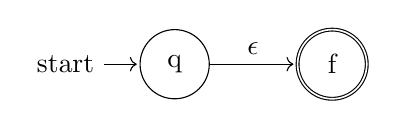
\begin{tikzpicture}[shorten >=1pt,node distance=2cm,on grid,auto]
            \node[state,initial] (q_0)   {q};
            \node[state,accepting] (q_1) [right=of q_0] {f};
            \path[->]
            (q_0) edge node { \( \epsilon \) } (q_1);
        \end{tikzpicture}
    \]
    \item if \texttt{a} is a regular expression, then the corresponding NFA is:
    \[
        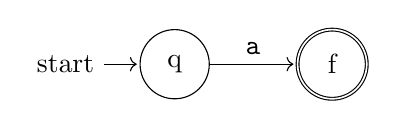
\begin{tikzpicture}[shorten >=1pt,node distance=2cm,on grid,auto]
            \node[state,initial] (q_0)   {q};
            \node[state,accepting] (q_1) [right=of q_0] {f};
            \path[->]
            (q_0) edge node { \texttt{a} } (q_1);
        \end{tikzpicture}
    \]
    \item The NFA of \texttt{(s)} is the same as the NFA of \texttt{s}.
    \item The NFA of \texttt{r|s} (Given \texttt{NFA{(s)}} and \texttt{NFA{(r)}}) is:
    \[
        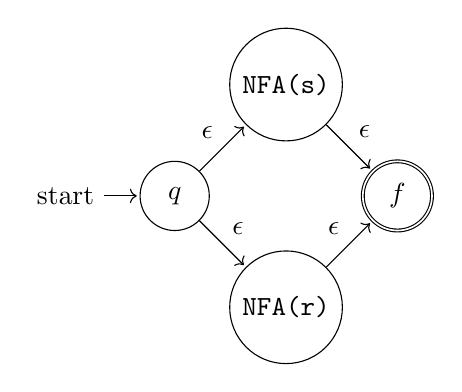
\begin{tikzpicture}[shorten >=1pt,node distance=2cm,on grid,auto]
            \node[state,initial] (q_0) {$q$};
            \node[state] (q_1) [above right=of q_0] {\texttt{NFA(s)}};
            \node[state] (q_2) [below right=of q_0] {\texttt{NFA(r)}};
            \node[state, accepting] (q_3) [below right=of q_1] {$f$};
            \path[->]
            (q_0) edge node {$\epsilon$} (q_1)
            (q_0) edge node {$\epsilon$} (q_2)
            (q_1) edge node {$\epsilon$} (q_3)
            (q_2) edge node {$\epsilon$} (q_3);
        \end{tikzpicture}
    \]
\end{enumerate}

\pagebreak

\end{document}